\documentclass[11pt,a4paper]{article}
\usepackage[a4paper, total={7in, 10.25in}]{geometry}


\usepackage{color}
\usepackage{graphicx}
\usepackage{wrapfig}
\usepackage{fancyhdr}
\usepackage{tocloft}
\usepackage{multicol}
\usepackage{hyperref}
\usepackage{tabularx}
\usepackage{array}
\usepackage[export]{adjustbox}
\usepackage{listings}
\usepackage{xcolor}
    \definecolor{codegreen}{rgb}{0,0.6,0}
    \definecolor{codegray}{rgb}{0.5,0.5,0.5}
    \definecolor{codepurple}{rgb}{0.58,0,0.82}
    \definecolor{backcolour}{rgb}{1,1,1}

    \lstdefinestyle{mystyle}{
        backgroundcolor=\color{backcolour},   
        commentstyle=\color{codegreen},
        keywordstyle=\color{magenta},
        numberstyle=\tiny\color{codegray},
        stringstyle=\color{codepurple},
        basicstyle=\ttfamily\footnotesize,
        breakatwhitespace=false,         
        breaklines=true,                 
        captionpos=b,                    
        keepspaces=false,                 
        numbers=left,                    
        numbersep=5pt,                  
        showspaces=false,                
        showstringspaces=false,
        showtabs=false,                  
        tabsize=2
    }



\renewcommand{\cftsecleader}{\cftdotfill{\cftdotsep}}
\graphicspath{ {./images/} }
\hypersetup{
    colorlinks=true,
    linkcolor=blue,
    citecolor=black,
    filecolor=magenta,      
    urlcolor=cyan,
    pdftitle={Overleaf Example},
    pdfpagemode=FullScreen,
    }
\pagestyle{fancy}
\setlength{\headheight}{18pt}
\fancyhead[L]{\textit{EN3160 Image Processing and Machine Vision : Assignment 02}}
\fancyfoot[L]{\textit{Department of Electronic and Telecommunication \\University of Moratuwa}}

\title{DEPARTMENT OF ELECTRONIC AND TELECOMMUNICATION
UNIVERSITY OF MORATUWA

{\textsf{EN3160 : Image processing and Machine Vision : Fitting and Alignment}}}

\author{200686J : Vishagar A.}

\begin{document}

\twocolumn

\maketitle

\section{Question 01}
In this question we are supposed to detect blobs in a given image. 
Blob detection is used to identify areas or objects that share characteristics like color, intensity, or texture. 
They distinguish out from their surroundings due to their homogenous characteristics.

The Laplacian of Gaussians (LoG), which uses a two-step procedure to improve features and find edges. 
The image is first smoothed using a Gaussian filter to reduces nois and highlights important structures. 
The Laplacian operator will draw attention to the areas where intensity changes have place.
By changing the valueis of $\sigma$ and threshold values we can detect blobs accurately.
And generally blobs are the superpositioned ripple gained from LoG.

And the Laplacian of Gaussian (LoG) is defined as follows.

\begin{equation}
    \nabla^2G(x,y) = \frac{1}{2\pi\sigma^2}(\frac{x^2+y^2-2\sigma^2}{\sigma^4})e^{-\frac{x^2+y^2}{2\sigma^2}}
\end{equation}

And following is the code for the implementation of LoG.

\lstset{style=mystyle}
\lstinputlisting[language=Python]{code1.py}

{\begin{figure}[h]
    \centering
    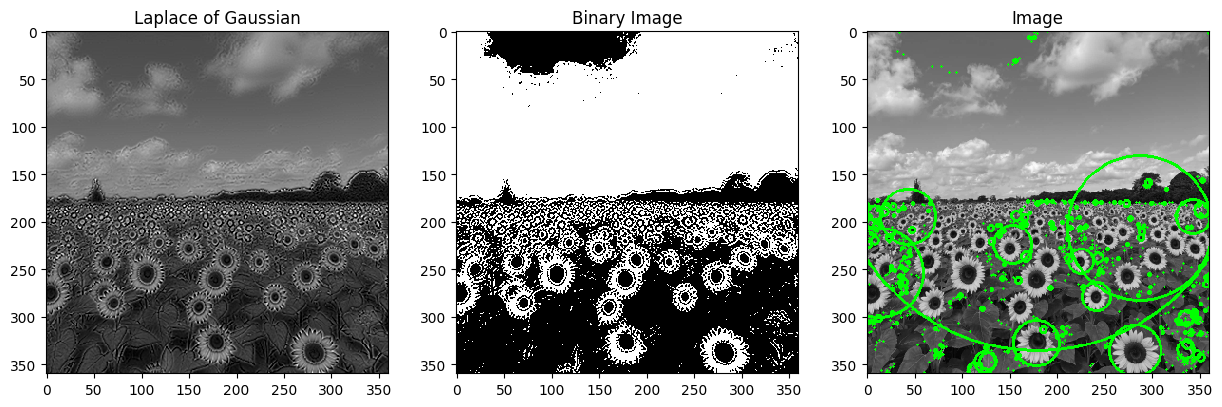
\includegraphics[width=1.0\linewidth]{images/1.png}
    \caption{LoG, thresholded LoG and detected blobs}
\end{figure}}

{\begin{figure}[h]
    \centering
    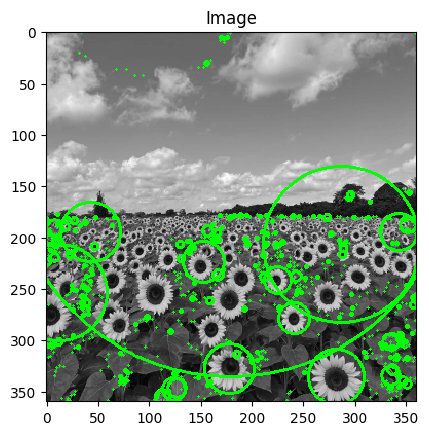
\includegraphics[width=0.825\linewidth]{images/12.png}
    \caption{Detected blobs }
\end{figure}}

\newpage
\begin{itemize}
    \item Maximum radius got : 76
    \item Range of $\sigma$ values : 0.5, 0.6, 0.75, 1.0, 2.0, 3.0
    \item Selected $\sigma$ value : 0.6375
\end{itemize}

\section{Question 02}

In this question we are supposed to estimate a line and a circle for a noisy dataset using RANSAC algorithm.
RANSAC is an iterative method to estimate parameters of a mathematical model from a set of observed data that contains outliers.

Following will be the code for the implementation of RANSAC algorithm for predicting a line for a noisy dataset.

\lstset{style=mystyle}
\lstinputlisting[language=Python]{code2.py}

\newpage

{\begin{figure}[h]
    \centering
    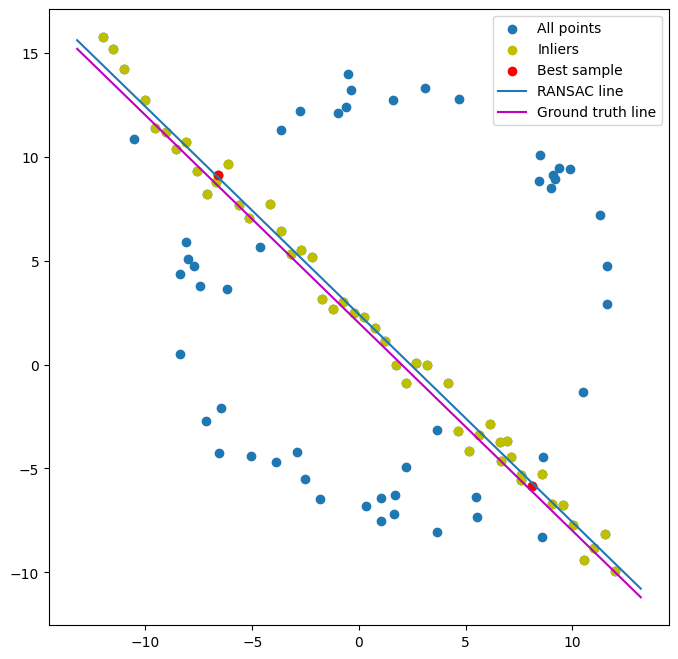
\includegraphics[width=0.75\linewidth]{images/2.png}
    \caption{Best fit line for the noisy dataset}
\end{figure}}

Code for estimating the circle

\lstset{style=mystyle}
\lstinputlisting[language=Python]{code3.py}

{\begin{figure}[h]
    \centering
    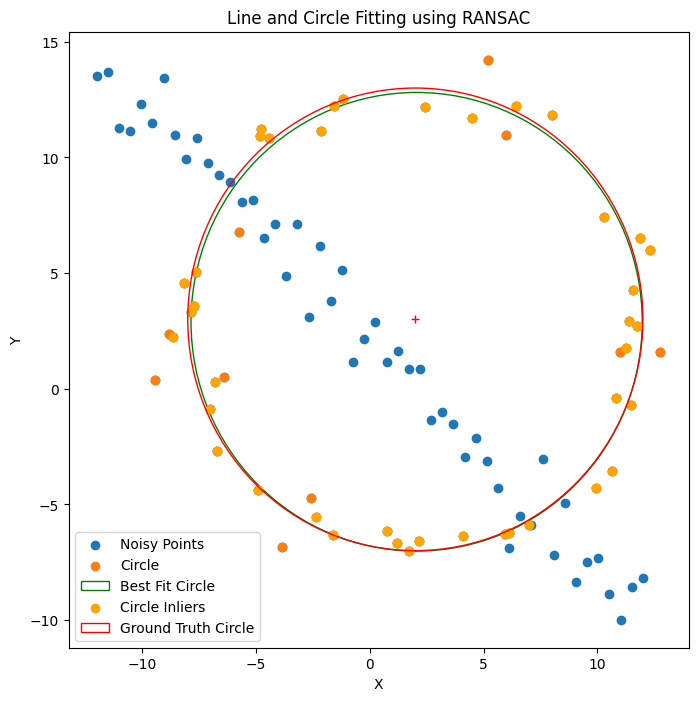
\includegraphics[width=0.75\linewidth]{images/22.png}
    \caption{Best fit circle for the noisy dataset}
\end{figure}}

\newpage

{\begin{figure}[h]
    \centering
    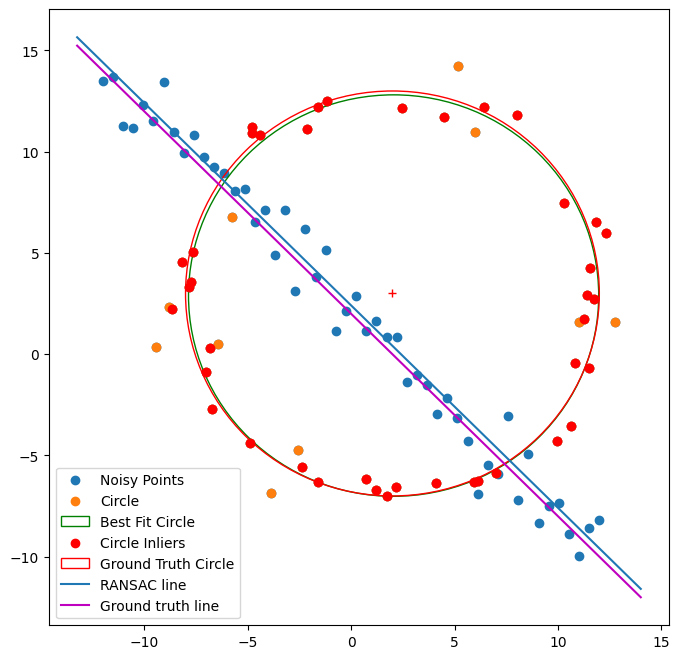
\includegraphics[width=1.0\linewidth]{images/23.png}
    \caption{Best fit and Grown truth line and circle.}
\end{figure}}

\subsection{Answer for part (d)}

In this case we are doing RANSAC fit for the line and subtract it from the noisy points and then we are proceeding with the fit for circle. Because of this RANSAC the circle inliers and creates a better fit for the circle by choosing random points.

But if we perform the ransac fit for the circle first, it will select some rondom points from the line inliers also. Because of this RANSAC can predict erroneous fits.
\section{Question 03}
This question is about wrapping one figure and superimposing it to another image.

\lstset{style=mystyle}
\lstinputlisting[language=Python]{code4.py}

{\begin{figure}[h]
    \centering
    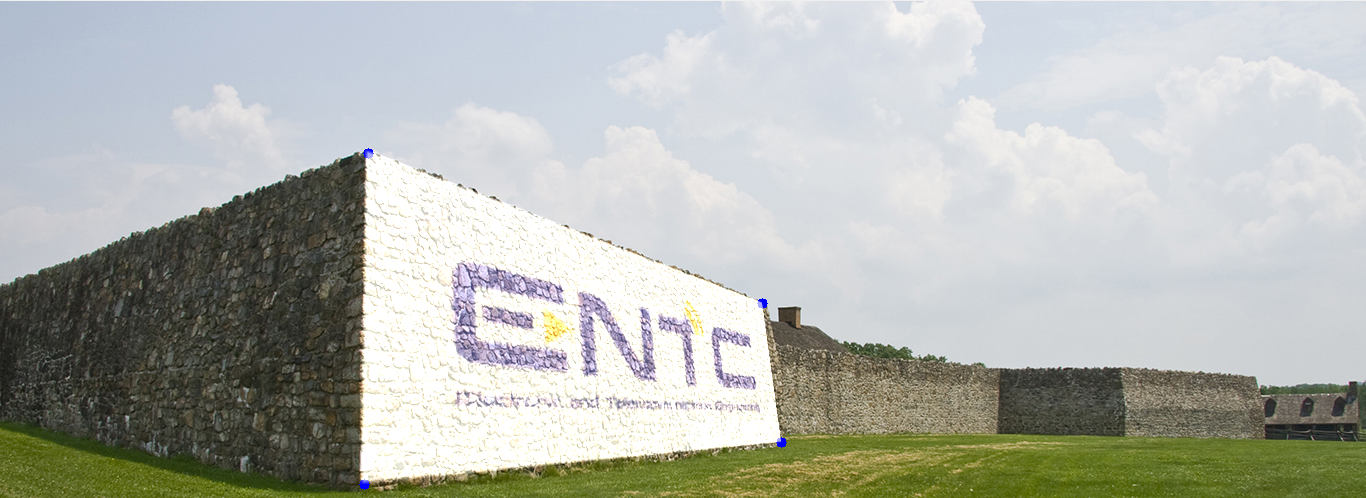
\includegraphics[width=1.0\linewidth]{images/3.png}
    \caption{Superposition Example 01}
\end{figure}}

{\begin{figure}[h]
    \centering
    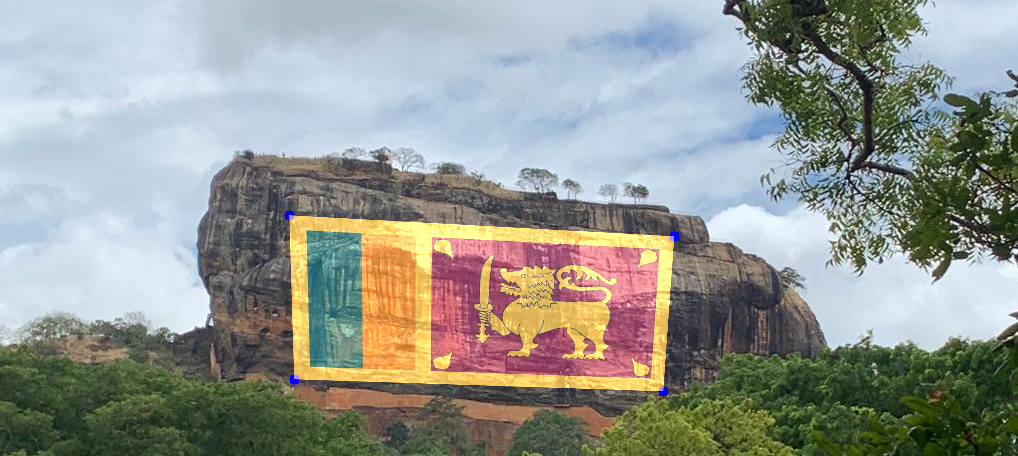
\includegraphics[width=1.0\linewidth]{images/4.png}
    \caption{Superposition Example 02}
\end{figure}}


\section{Question 04}

In this question we are supposed to stich to images together. For this we need to create keypoints and descriptors for both images and then match them using a matcher. Then we need to find the homography matrix and warp the image to the other image. We can SIFT for creating keypoints and descriptors. And we can use RANSAC for finding the best homography matrix along with BFmatcher for matching the descriptors.\\

Following will be the implementation for creating keypoints and descriptors.

\lstset{style=mystyle}
\lstinputlisting[language=Python]{code5.py}

\newpage

{\begin{figure}[h]
    \centering
    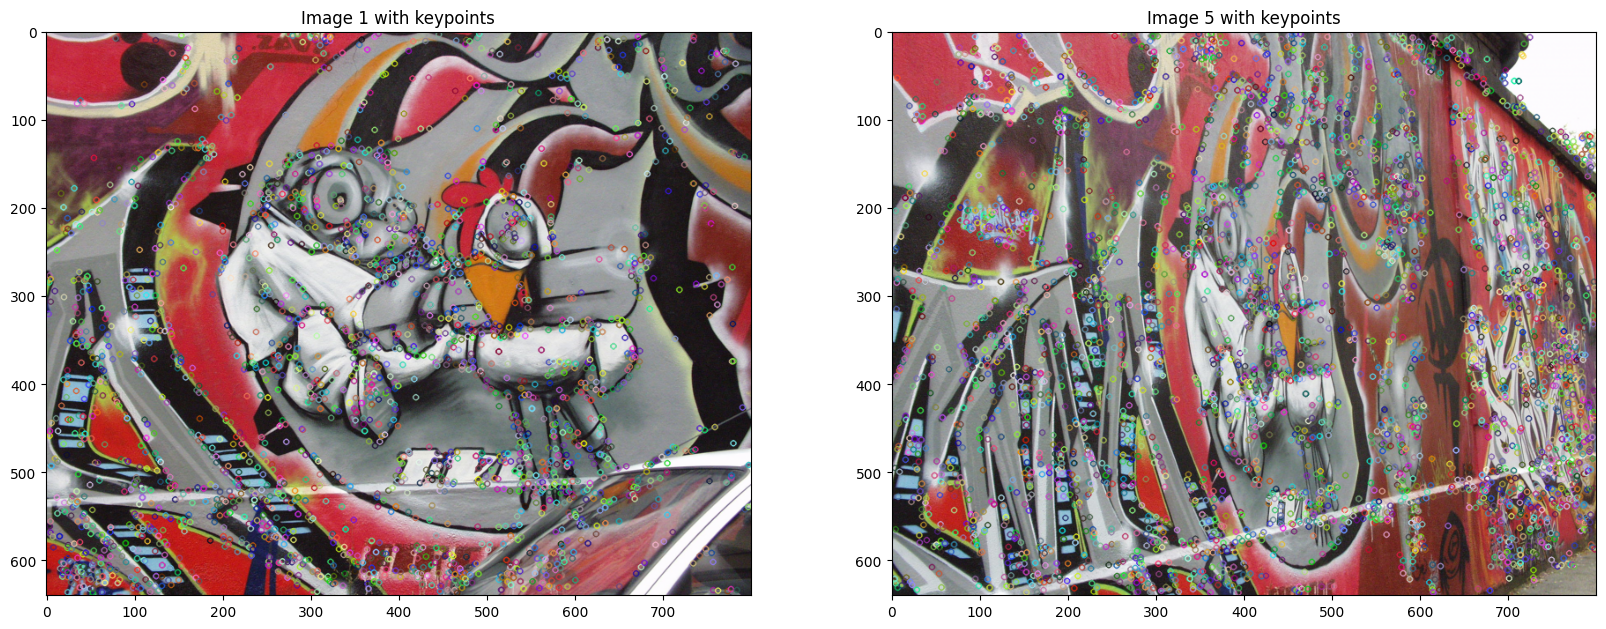
\includegraphics[width=1.0\linewidth]{images/5.png}
    \caption{EDetected Keypoints}
\end{figure}}

And the keypoints were mathched using BFmatcher and the homography matrix was found using RANSAC. And the following is the code for that.

\lstset{style=mystyle}
\lstinputlisting[language=Python]{code6.py}

{\begin{figure}[h]
    \centering
    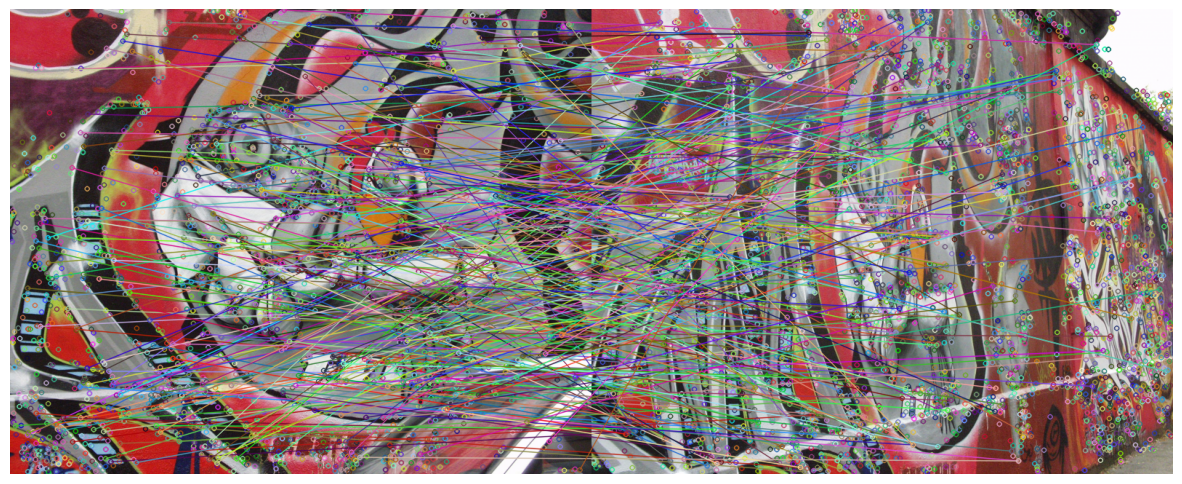
\includegraphics[width=1.0\linewidth]{images/52.png}
    \caption{Matched Keypoints}
\end{figure}}

And I got the following matrix as my homography matrix. for the above code.
\[
\left[
\begin{array}{ccc}
    -3.99590 \times 10^{-1} & 1.98442 \times 10^{-1} & 1.73728 \times 10^{2} \\
    -9.24469 \times 10^{-1} & 4.81236 \times 10^{-1} & 3.95571 \times 10^{2} \\
    -2.32774 \times 10^{-3} & 1.19405 \times 10^{-3} & 1.00000
\end{array}
\right]
\]

\lstset{style=mystyle}
\lstinputlisting[language=Python]{code7.py}

{\begin{figure}[h]
    \centering
    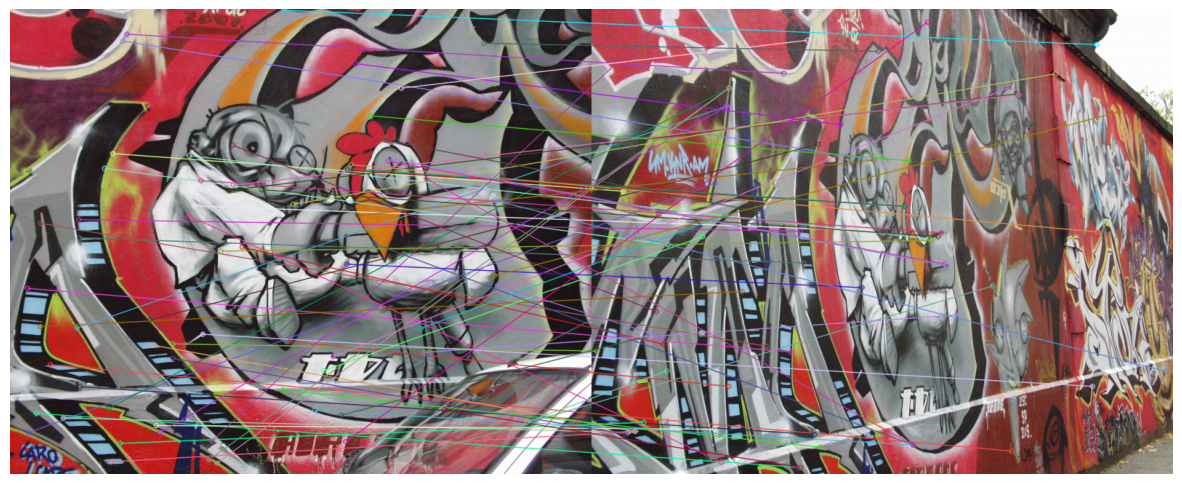
\includegraphics[width=1.0\linewidth]{images/53.png}
    \caption{Matched Keypoints using RANSAC}
\end{figure}}

And I tried to stich the matching keypoints but I could not able to accomplish it.

{\begin{figure}[h]
    \centering
    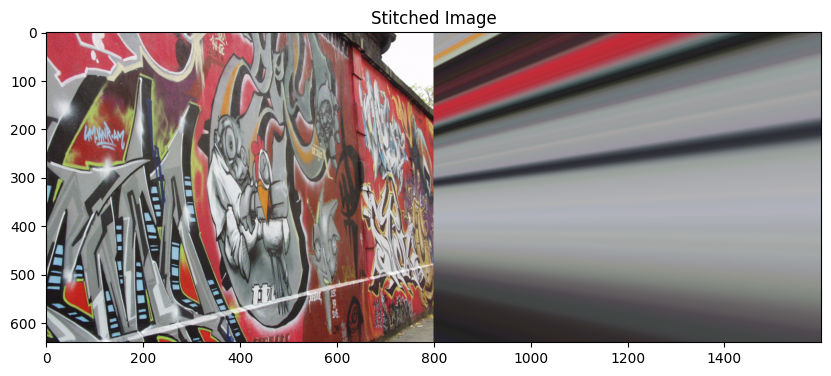
\includegraphics[width=1.0\linewidth]{images/54.png}
    \caption{Stiched Image}
\end{figure}}


\section{References}

\begin{itemize}
    \item \href{https://numpy.org/doc/}{Numpy Documentation}
    \item \href{https://docs.opencv.org/4.x/}{OpenCV Documentation}
    % \item \href{ }{Github/EN3160_Assignment_01}
   
\end{itemize}

\section{Github Repository}

Following is the link to my Github repository for this assignment.\\

\href{https://github.com/Vgr20/EN_3160_Assignment_02.git}{Github/EN160\_Assignment\_02}


% \lstset{style=mystyle}
% \lstinputlisting[language=Octave]{code2.py}

\end{document}




%%%%%%%%%%%%%%%%%%%%%%%%%%%%%%%%%%%%%%%%%%%%%%%%%%%%%%%%%%%%%%%%%%%%%%%%%%%%%%%%%%%%%%%%%%%%%%%%%%%%%%%%%%%%%%%%%%%%%%%%%%%%%%%%%%%%%%%%%%%%%%%%%%%%%%%%%%%%%%%%%%%%%%%%%%

% {\begin{center}
% \begin{tabular}{ | m{1.85cm} | m{0.85cm}| m{0.85cm} | m{0.85cm} | m{0.85cm} | m{0.85cm} | } 
%  \hline
%  Objectives& Weight & Design 01 & Design 02 & Design 03 & Design 04 \\  
%  \hline\hline
%  Efficiency & 10 & 7 & 8 & 8 & 9 \\
%  \hline
%  Mobility & 10 & 7 & 9 & 8 & 8 \\
%  \hline
%  Easy Maintenance & 10 & 7 & 6 & 5 & 8 \\
%  \hline
%  Refilling accessibility & 5 & 3 & 3 & 2 & 4 \\
%  \hline
%  Durability & 5 & 2 & 3 & 3 & 2 \\
%  \hline
%  Manufacture cost & 5 & 3 & 3 & 2 & 3 \\
%  \hline
%  Overall Look & 5 & 2 & 3 & 5 & 2 \\
%  \hline
%  \hline
%  Total & 50 & 31 & 35 & 33 & 36 \\
%  \hline
 
% \end{tabular}
% \end{center}}

%%%%%%%%%%%%%%%%%%%%%%%%%%%%%%%%%%%%%%%%%%%%%%%%%%%%%%%%%%%%%%%%%%%%%%%%%%%%%%%%%%%%%%%%%%%%%%%%%%%%%%%%%%%%%%%%%%%%%%%%%%%%%%%%%%%%%%%%%%%%%%%%%%%%%%%%%%%%%%%%%%%%%%%%%%


% \begin{center}
% \begin{tabular}{ | m{2cm} | m{5cm}| m{2cm} | m{6cm} | } 

%  \hline
%  Part Name & Description & Supplier & Part Link\\  
%  \hline\hline
%  NE555P & 8-pin Precise timer & Texas Instruments & \href{https://www.lcsc.com/product-detail/Timers-Clock-Oscillators_Texas-Instruments-NE555P_C46749.html}{NE555p data sheet}\\
%  \hline
%  2N2222A & Generic npn transistor & Slkor & \href{https://www.lcsc.com/product-detail/Bipolar-Transistors-BJT_Slkor-SLKORMICRO-Elec-2N2222A_C5330385.html}{2N2222A data sheet}\\
%  \hline
%   LM7805 & Linear voltage Regulators & LRC & \href{https://www.lcsc.com/product-detail/Linear-Voltage-Regulators-LDO_LRC-LR7805_C2846986.html}{Lm7805 Data sheet}\\
%  \hline
%   HC sr501 & Passive IR sensor & HC & \href{https://www.lcsc.com/product-detail/Timers-Clock-Oscillators_Texas-Instruments-NE555P_C46749.html}{HC sr501 data sheet}\\
%  \hline
%   KNSCHA ZE11000UF & 1000uF Capacitor & KNSCHA & \href{https://www.lcsc.com/product-detail/Solid-Capacitors_KNSCHA-ZE11000UF35V119EC0014_C2992586.html}{Capacitor data sheet}\\
%  \hline
%   Resistors & Resistors with different values & Texas Instruments & \href{https://www.lcsc.com/search?q=resistors%20through%20hole}{Through hole resistors}\\
%  \hline
 
% \end{tabular}  
% \end{center}
%%%%%%%%%%%%%%%%%%%%%%%%%%%%%%%%%%%%%%%%%%%%%%%%%%%%%%%%%%%%%%%%%%%%%%%%%%%%%%%%%%%%%%%%%%%%%%%%%%%%%%%%%%%%%%%%%%%%%%%%%%%%%%%%%%%%%%%%%%%%%%%%%%%%%%%%%%%%%%%%%%%%%%%%%%